\chapter{Dokumentacja projektowa}

\section{Architektura systemu}
Wytworzony w ramach pracy system jest aplikacją webową, która korzysta z bazy danych do odczytu i zapisu niezbędnych informacji. Z systemu będą korzystać cztery, wcześniej omówione, rodzaje użytkowników poprzez interfejs WWW. Dodatkowo system został zaprojektowany w taki sposób, aby była możliwość rozbudowy o dodatkowe zdalne aplikacje klienckie umożliwiające komunikację z systemem. System wraz z bazą danych znajdują się w kontenerze Dockera.

Jak wiadomo, połączenie ze zdalnymi klientami nie jest gwarantowane, co skłania do zastosowania mechanizmu komunikacji Java Message Service (JMS). Jednak pomimo, że połączenie nie jest ani stabilne, ani nawet w ogóle nie wiadomo czy zostało nawiązane, zależy nam, aby informować użytkowników o różnego rodzaju błędach, lub przesyłać im dane na bieżąco. Co prawda JMS umożliwia realizację tego zadania lecz do komunikacji z samodzielną aplikacją zostały udostępnione inne ścieżki komunikacji. 

Pierwsza z nich to warstwa usługi REST. Dzięki takiemu rozwiązaniu z aplikacją może komunikować się dowolny system niezależnie od tego w jakim języku został napisany. Warstwa ta nie została zaimplementowana w całości, lecz jedynie jako fragment funkcjonalności w celu zobrazowania komunikacji ze zdalnymi klientami.

Kolejna ścieżka komunikacji to zdalny interfejs komponentu EJB (Enterprise JavaBean). Mechanizm ten wprowadza możliwość komunikacji asynchronicznej z aplikacją. Jest on jednak ograniczony tylko do klientów napisanych w języku Java.

Wyżej wymienione rozwiązania stanowią warstwę do komunikacji z aplikacjami klienckimi. Kolejnym krokiem było zaprojektowanie warstwy do komunikacji z klientem WWW. Co prawda warstwa REST spełniałaby te wymagania, lecz w tym celu posłużymy się, specjalnie zaprojektowaną do tego rodzaju zadań, technologią JavaServer Faces (JSF). Rozwiązanie to pozwoli nam zaimplementować dodatkową warstwę, dedykowaną specjalnie dla interfejsu WWW. Warstwa ta to tzw. komponenty Java Beans zwane również Backing Beans (BB). Rysunek \ref{fig:diagsys} przedstawia diagram systemowy aplikacji:

\begin{figure}[h!]
	\centering
	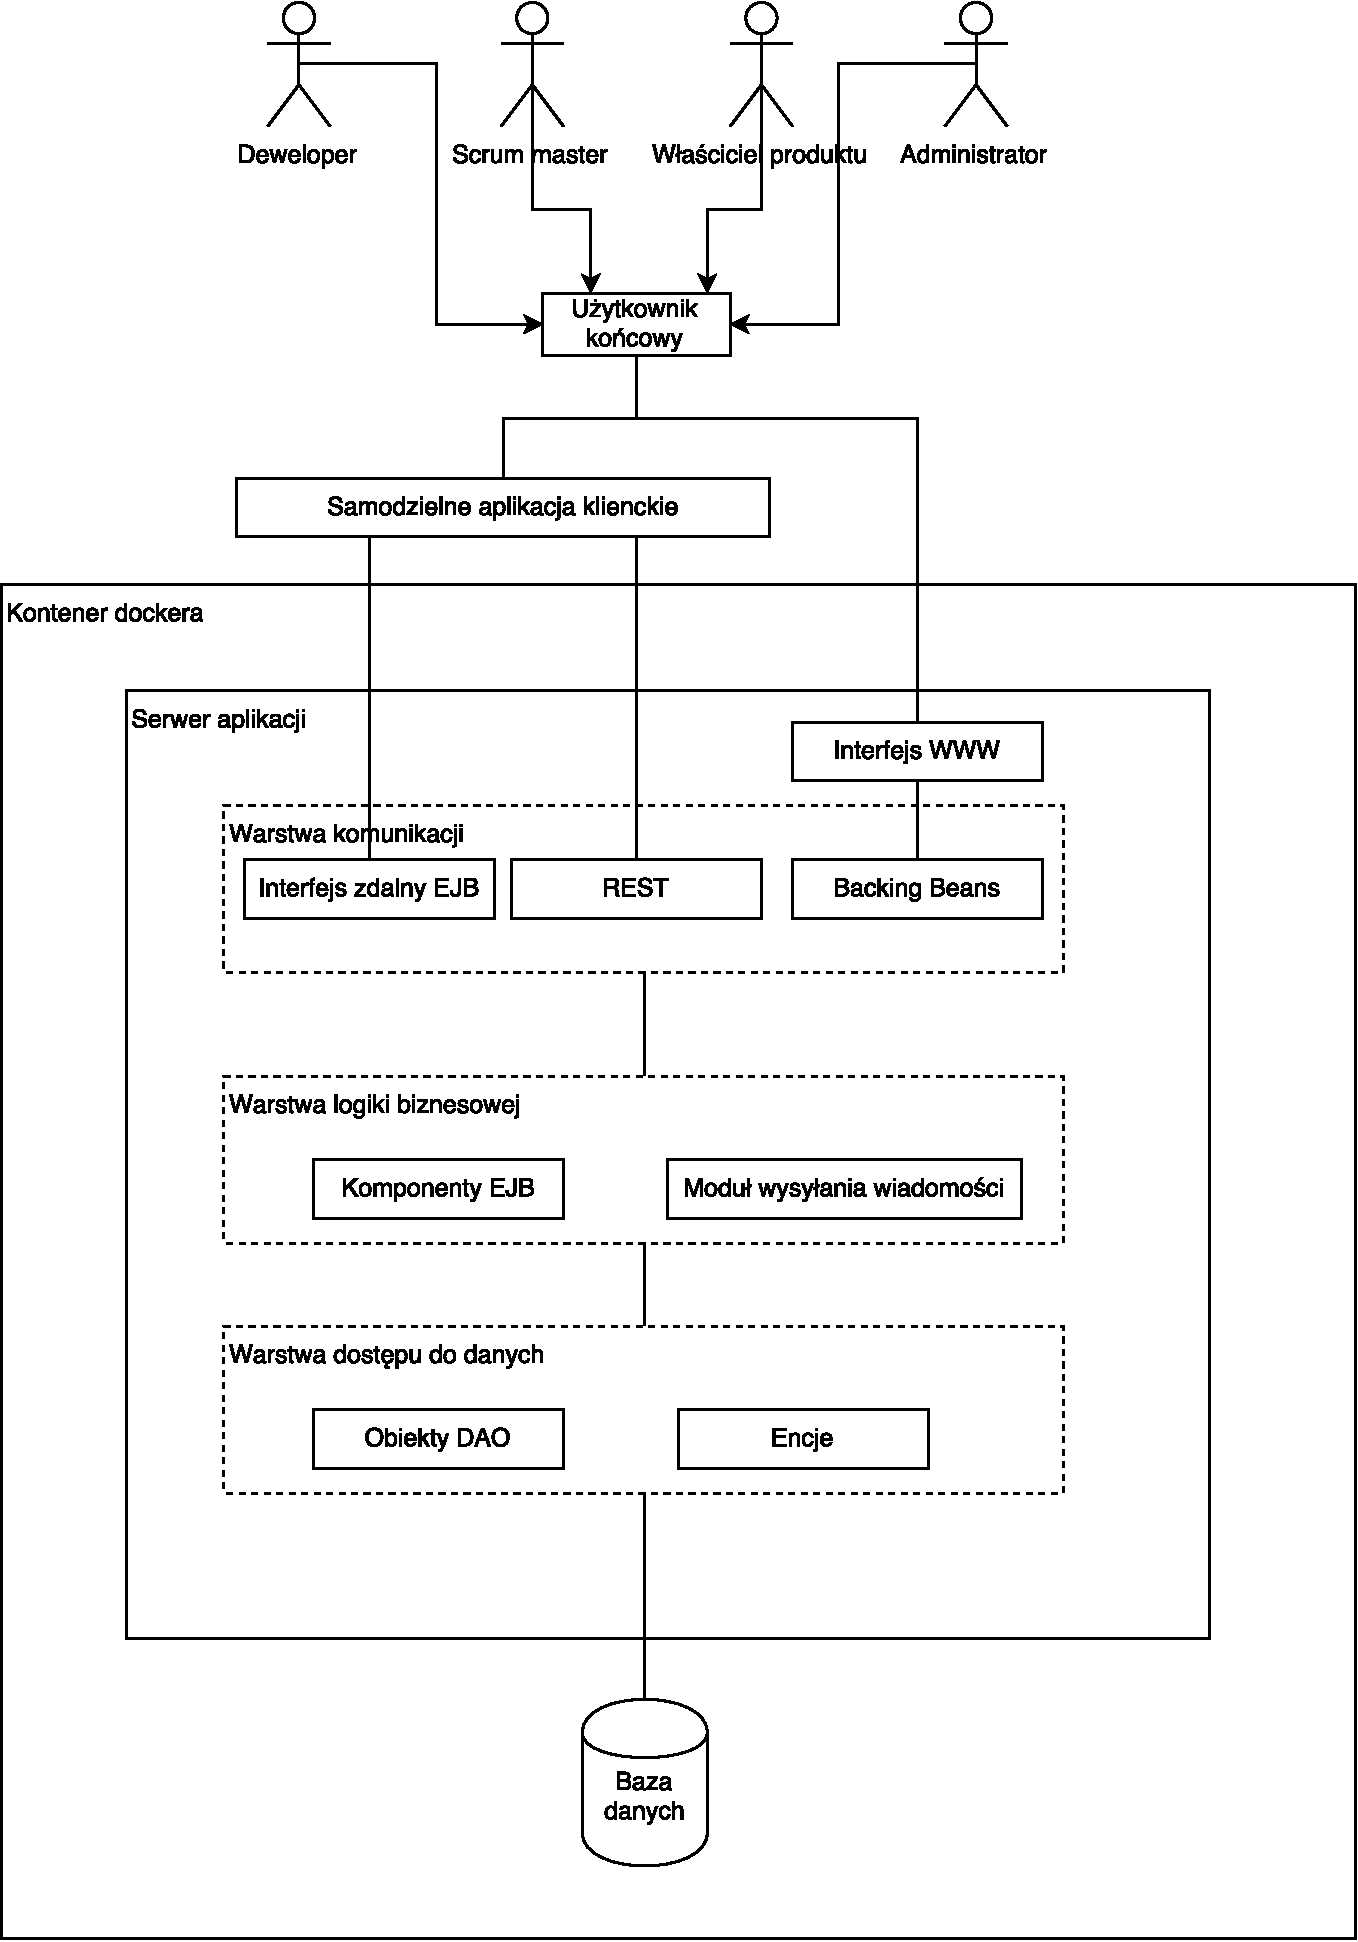
\includegraphics[width=13.5cm]{rysunki/diagsys.pdf}	
	\caption{Diagram systemowy aplikacji}
	\label{fig:diagsys}
\end{figure}

Jak wiadomo, interfejsy graficzne, a co za tym idzie – sposób ich obsługi będą się różniły w zależności od klienta. Najważniejszą różnicą będzie sposób walidacji danych oraz obsługi błędów. W samodzielnej aplikacji klienckiej walidacja danych oraz obsługa błędów powinna wystąpić możliwie szybko, aby nie generować zbędnego ruchu sieciowego. Jeżeli w trakcie przetwarzania żądania wystąpią jakiekolwiek błędy, to powinny one zostać zamienione na wyjątki aplikacji oraz być przekazane do klienta. Również w aplikacji WWW walidacja danych wejściowych powinna znajdować się na poziomie klienta. Jednak nie można wykluczyć sytuacji, w której błędy pojawią się po stronie serwera nawet po poprawnej walidacji danych. Z tego względu błędy powinny być konwertowane po stronie serwera (przez dodatkową warstwę obsługi JSF) na obiekty typu FaceMessage i dodawane bezpośrednio do kontekstu aplikacji WWW. 

Wymagania odnośnie walidacji oraz obsługi błędów mogą skłaniać do wprowadzenia dodatkowej warstwy w architekturze systemu. Nie mniej jednak taka warstwa nie została wprowadzona, gdyż spowodowało by to nadmierny przyrost klas oraz niepotrzebne uogólnienie systemu. Zamiast tego logika biznesowa generuje wyjątki aplikacji, gdy zajdzie taka potrzeba oraz przekazuje je warstwie wyżej lub klientom, które wywołują dane komponenty logiki biznesowej. Oznacza to tyle, że obsługa błędów aplikacji w samodzielnej aplikacji Javy powinna być zaimplementowana po stronie samej aplikacji, natomiast interfejs WWW posiada dodatkową warstwę w postaci komponentów JavaBeans, które takową obsługę zapewnią. 

\subsection{Identyfikacja komponentów biznesowych}
W oparciu o artefakty metodyki Scrum oraz wymagania funkcjonalne z systemu wyłaniają się następujące komponenty biznesowe:

\textit{Deweloper} -- użytkownik aplikacji, może przeglądać oraz modyfikować \textit{zadania} w \textit{projektach}, do których należy.

\textit{Scrum master} -- użytkownik aplikacji, jest przypisany do jednego lub wielu \textit{zespołów}.

\textit{Właściciel produktu} -- użytkownik aplikacji, jest przypisany tylko do jednego \textit{projektu}.

\textit{Administrator} -- użytkownik aplikacji, zarządza całym systemem. Może tworzyć nowe \textit{projekty} oraz \textit{zespoły}.

\textit{Zespół} -- zbiór \textit{deweloperów}, może być powiązany z \textit{projektem}.

\textit{Projekt} -- zbiór \textit{zadań}, posiada \textit{właściciela produktu}.

\textit{Sprint} -- jest tworzony przez  \textit{scrum mastera}. Posiada \textit{story}.

\textit{Story} -- jest agregatem \textit{zadań}.

\textit{Backlog} -- przynależy do \textit{projektu}, posiada \textit{zadania}.

\textit{Zadanie} -- jest tworzone przez \textit{użytkowników}.


Należy wspomnieć, iż jest to częściowy opis obiektów biznesowych, który ma na celu zobrazowanie procesu powstawania aplikacji. Wyczerpujący opis tych obiektów byłby zbyt rozległy i nie jest on meritum części opisowej pracy. Aby zobrazować wpływ poszczególnych jednostek biznesowych oraz ich wzajemne relacje należy przedstawić ich diagram UML:
\begin{figure}[h!]
	\centering
	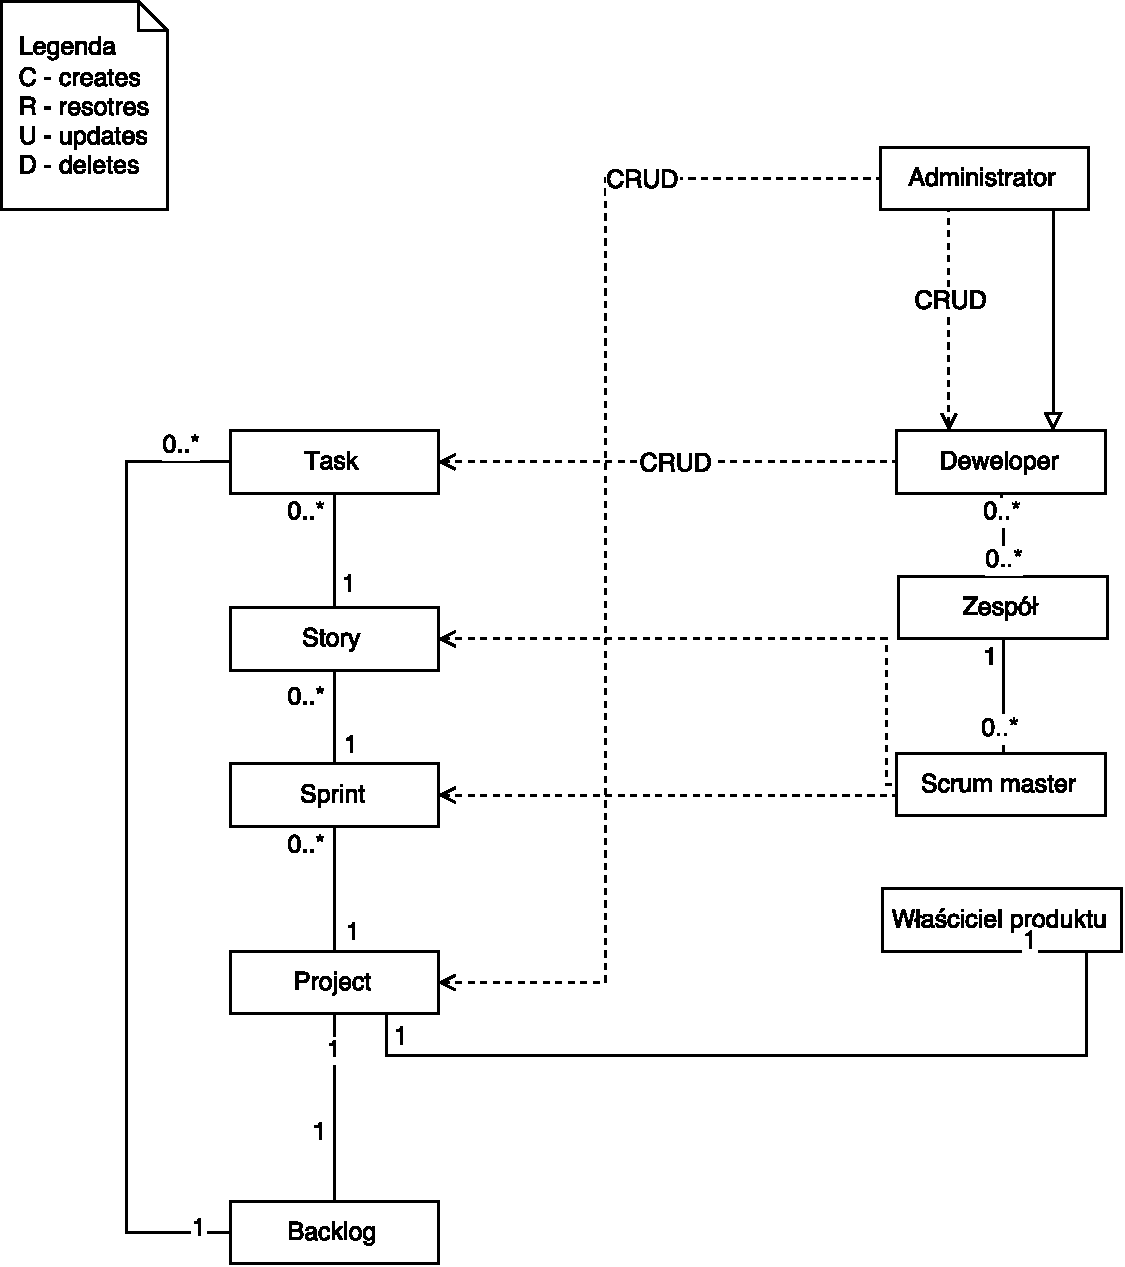
\includegraphics[width=15cm]{rysunki/diaguml.pdf}	
	\caption{Diagram jednostek biznesowych}
	\label{fig:diaguml}
\end{figure}

\section{Struktura projektu}
W poprzedniej sekcji została opisana ogólna architektura systemu umożliwiająca pogląd na całą aplikację. Teraz zostaną opisane wybrane komponenty. Zanim jednak to zrobimy zostanie przedstawiony bardziej szczegółowy diagram jednostek biznesowych, który uwzględnia funkcje, jakie można wykonywać w systemie. Diagram powstał w oparciu o wymagania funkcjonalne, które szczegółowo opisują, co dany użytkownik może robić, oraz o identyfikację komponentów biznesowych omówionych wcześniej. Także i tutaj należy zwrócić uwagę, iż nie jest to wyczerpujący diagram klas opracowanych w systemie:
\begin{figure}[h!]
	\centering
	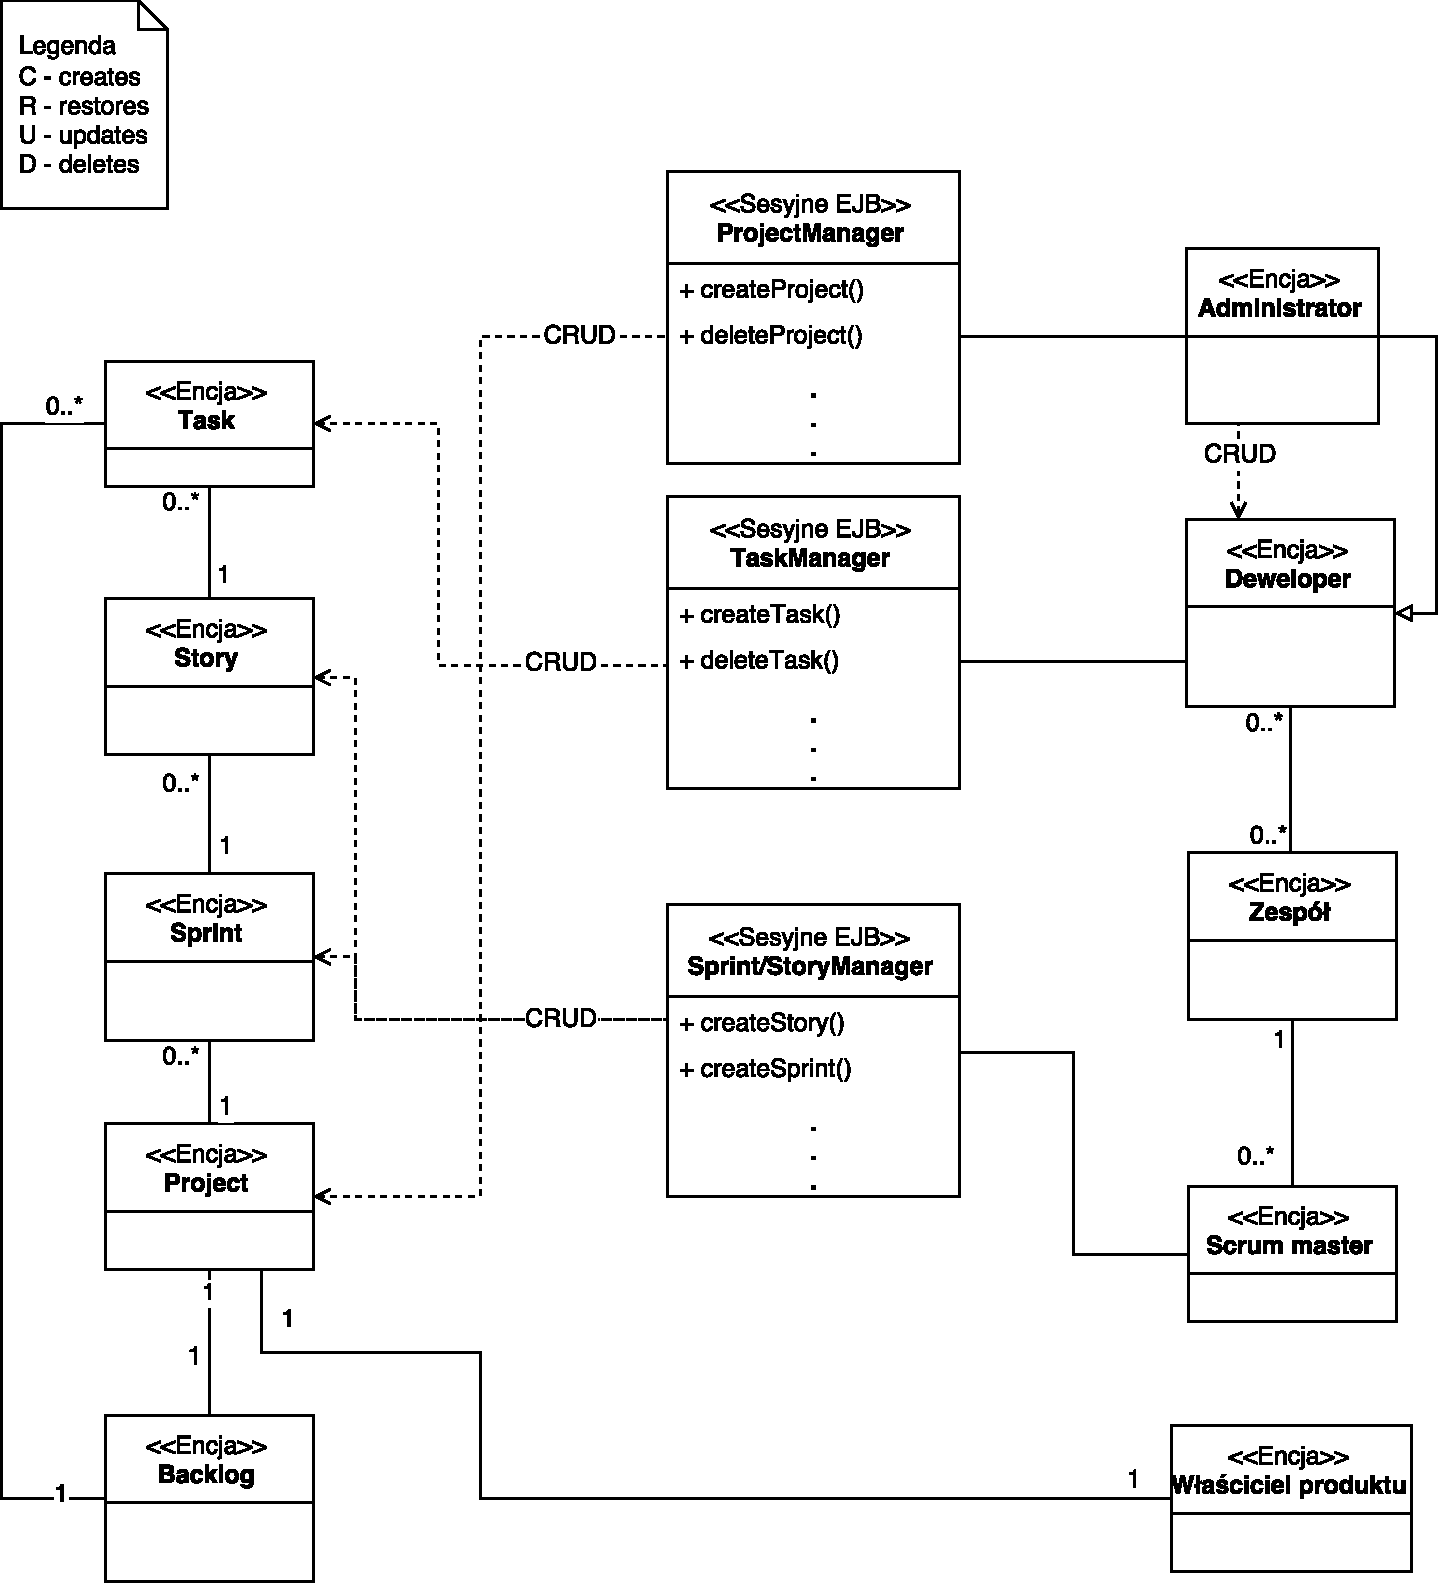
\includegraphics[width=15cm]{rysunki/diagdetailuml.pdf}	
	\caption{Szczegółowy diagram wybranych klas}
	\label{fig:diagdetailuml}
\end{figure}

\subsection{Klasyfikacja komponentów EJB}
W tej sekcji zostaną opisane komponenty EJB używane w aplikacji oraz takie, które nie zostały użyte wraz z podaniem argumentów dlaczego je pominięto.

\subsubsection{Komponenty encyjne}
Reprezentują rekordy utrwalone w bazie danych. Komponenty encyjne mogą być używane do reprezentowania rzeczowników lub rzeczy z opisu funkcjonalnego. Jeżeli jednostka biznesowa posiada odpowiednik w rzeczywistości, to jest to prawdopodobnie komponent encyjny.

\subsubsection{Komponenty sesyjne}
Podczas gdy komponenty encyjne są rzeczami w aplikacji, komponenty sesyjne określają czynności jakie można na tych rzeczach wykonać. Są one jednostkami kontrolującymi procesy biznesowe. Zatem, aby wyodrębnić ten rodzaj komponentów należy się skupić na tym, co aplikacja może robić.
Przyglądając się diagramowi klas można zauważyć, że ProjectManager może wykonywać operacje Create Restore Update Delete (CRUD) na projektach.
Gdy w dowolnej aplikacji funkcjonalności skupiają się zazwyczaj wokół jednej lub więcej encji, to znaczy, że prawdopodobnie jest to komponent sesyjny. Ta reguła również tutaj ma swoje zastosowanie. Zostały utworzone odpowiednie komponenty sesyjne, które są swego rodzaju menedżerami spinającym funkcjonalności biznesowe, które są ze sobą powiązane. Ponieważ komponent sesyjny definiuje zbiór zachowań, to każde takie zachowanie można podporządkować jednej metodzie.

Głównym zadaniem aplikacji będzie przeglądanie projektów oraz zadań. W tym celu zostały utworzone odpowiednie komponenty sesyjne dla każdego rodzaju obiektu biznesowego, które jednak nie zostały przedstawione na szczegółowym diagramie, ze względu na ich obszerność. Każdy taki komponent posiada metody CRUD, które umożliwiają wykonywanie dowolnych operacji na tychże obiektach.

Tworzona aplikacja skupia się na zarządzaniu projektami, więc bez konfiguracji wstępnej – utworzenia użytkowników, przyznanie praw właściciela produktu, czy administratora  – zarządzanie, a nawet samo utworzenie projektu będzie nie możliwe. Ponieważ tymi rzeczami zajmuje się administrator, więc w działającym systemie musi istnieć już użytkownik z uprawnieniami administratora. Dzięki temu system jest gotowy do działania zaraz po uruchomieniu.

\subsubsection{Komponenty sterowane komunikatami}
Pomimo iż zostało postanowione, że w aplikacji nie będą użyte komponenty sterowane komunikatami, nic nie stoi na przeszkodzie, aby głębiej przemyśleć możliwość wykorzystania takich komponentów. Zastanówmy się, w jakich sytuacjach mogłyby one być korzystne.

Pierwszą rzeczą, która nasuwa się na myśl jest wykorzystanie MDB (Message Driven Bean) do generowania i wysyłania e-maili z hasłem po utworzeniu użytkownika. Taka wiadomość mogła by być rozgłoszona w systemie i dzięki temu różne komponenty mogłyby obsłużyć to zdarzenie. W systemie zrezygnowano jednak z tego typu technik.

Drugim możliwym zastosowaniem jest możliwość wysyłania rozgłoszeń w systemie. Jednak że aplikacja nie wprowadza funkcjonalności wiadomości systemowych również i tu ten komponent nie ma zastosowania.

Na tym etapie warto wspomnieć, że komponenty sterowane komunikatami można wprowadzić na każdym etapie udoskonalania projektu, jednak warto zwrócić uwagę na to, jak zachować odpowiedni stopień bezpieczeństwa przy tego typu komunikatach.

\section{Model bazy danych}
System korzysta z zewnętrznej bazy danych, której model jest przedstawiony na rysunku \ref{fig:modeldb}. Został on wygenerowany za pomocą testowej wersji programu DbSchema. Kolorem zielonym zostały oznaczone tabele dotyczące użytkowników oraz uprawnień. Niebieski kolor oznacza tabele złączeniowe, które nie mają odwzorowania w kodzie. Czerwone zaś to pozostałe struktury występujące w projekcie -- są to obiekty na których operują użytkownicy. Model bazy został wygenerowany bezpośrednio z klas Javy, za pomocą frameworka Hibernate oraz specyfikacji JPA (\textit{ang. Java Persistence API}).

\begin{sidewaysfigure}[h!]
	\centering
	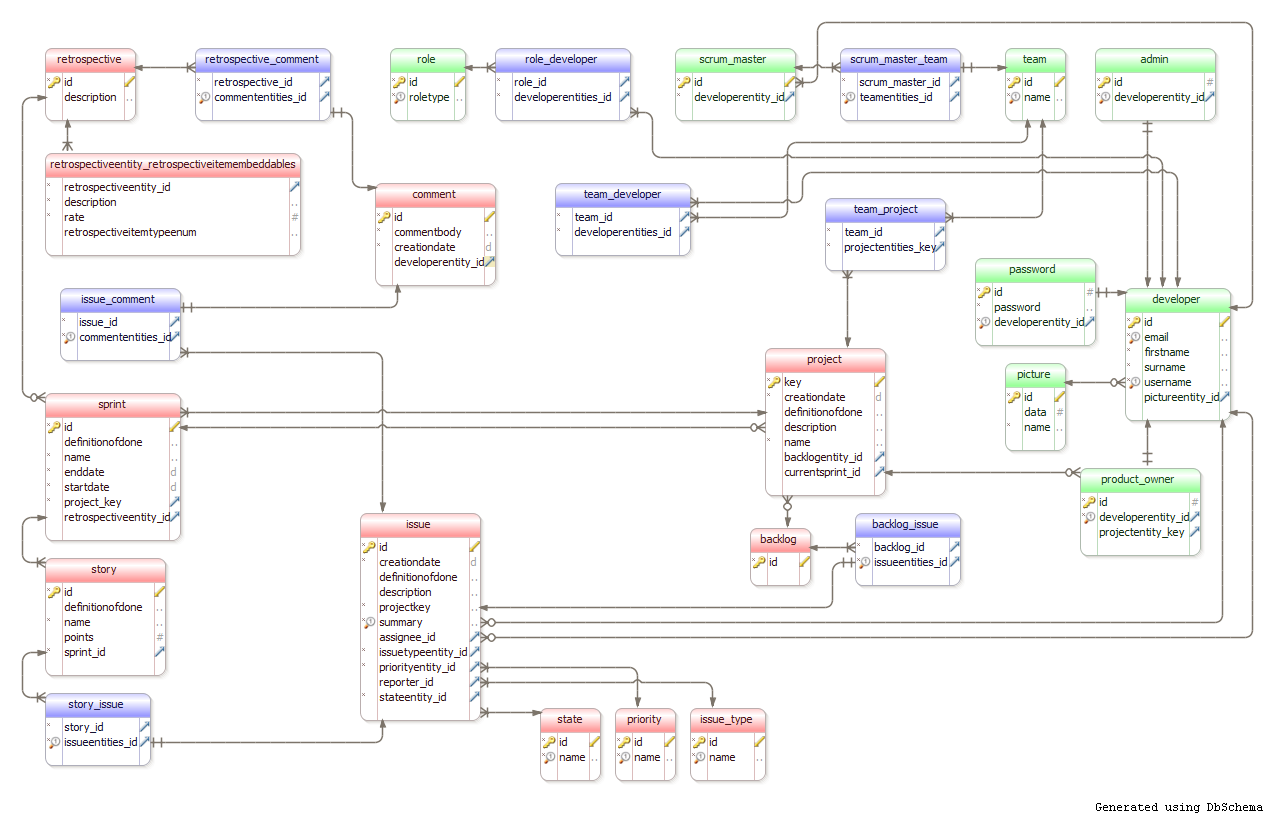
\includegraphics[width=25cm]{rysunki/modeldb.png}	
	\caption{Model bazy danych projektu scrumus}
	\label{fig:modeldb}
\end{sidewaysfigure}

\section{Szczegóły implementacji}
Przy omawianiu szczegółów implementacji przejdziemy przez cały zaprojektowany system w kierunku od bazy danych poprzez logikę biznesową, warstwę prezentacji a w następnym rozdziale przejdziemy do sposobu uruchomienia aplikacji wraz z opisem środowiska testowego i produkcyjnego, które w przypadku tego projektu stanowiły jedność. Zanim jednak przystąpimy do opisu poszczególnych warstw, w celu zrozumienia wszystkich omawianych zagadnień, warto zapoznać się ze strukturą plików i folderów w projekcie scrumus, która została przedstawiona na rysunku \ref{fig:struktura_intellij}.

\begin{figure}[tp]
	\centering
	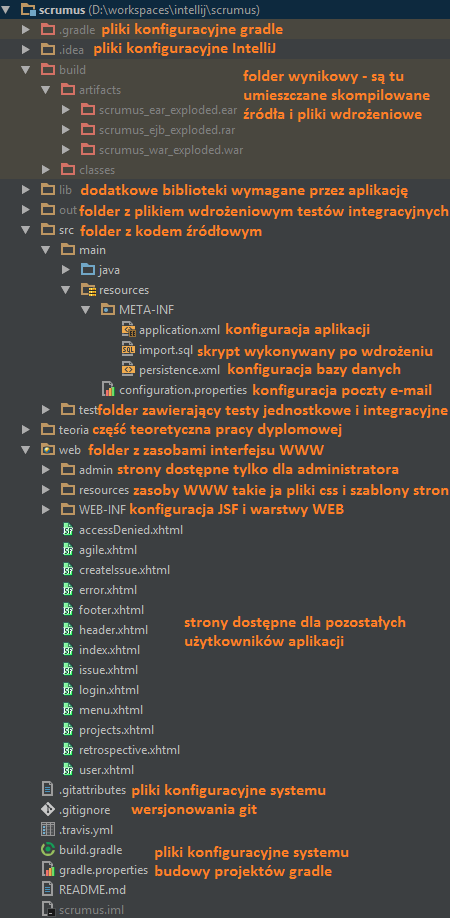
\includegraphics[width=12cm]{rysunki/struktura_intellij.png}	
	\caption{Struktura plików i folderów projektu scrumus}
	\label{fig:struktura_intellij}
\end{figure}

\subsection{Baza danych i model}
Model bazy danych został zaprojektowany w postaci klas Javy, tak zwanych encji, a następnie automatycznie wygenerowany za pomocą frameworka Hibernate. Dodatkowo zaraz po wdrożeniu aplikacji na serwer wykonywany jest skrypt SQL, który wprowadza do bazy testowe wartości i tworzy użytkowników z różnymi uprawnieniami. Przykładowy kod klasy encji został przedstawiony na listingu \ref{lis:encja}, a konfiguracja Hibernate na listingu~\ref{lis:konfiguracja_hibernate}.

\begin{lstlisting}[caption={Przykładowa klasa encji}, label=lis:encja, numbers=none]
@Data									 		// adnotacja lombok dodaje gettery
@NoArgsConstructor 				// settery oraz hashcode i equals
@Entity				  	 		 		// oznaczenie klasy jako encji
@Table(name = "project")  //nazwa tabeli w bazie danych
@NamedQueries({@NamedQuery(name = ProjectEntity.FIND_ALL, 
													 query = ProjectEntity.FIND_ALL_QUERY),
   							//pozostale zapytania uzywane przez DAO})
public class ProjectEntity {

// zapytania nazwane

// mapowanie
@Id
@Column(length = 8, nullable = false, unique = true)
private String key;

// pozostale pola
}\end{lstlisting}
\newpage
\begin{lstlisting}[caption={Konfiguracja Hibernate}, label=lis:konfiguracja_hibernate, numbers=none]
<?xml version="1.0" encoding="UTF-8"?>
<persistence xmlns="http://java.sun.com/xml/ns/persistence"
					 	 version="2.0">
	<persistence-unit name="PostgresDS">
		<jta-data-source>java:jboss/datasources/PostgresDS</jta-data-source>
		<properties>
			<property name="hibernate.show_sql" 
								value="false"/>
			<property name="hibernate.format_sql" 
								value="true"/>
			<property name="hibernate.dialect" 
								value="org.hibernate.dialect.PostgreSQLDialect"/>
			<property name="hibernate.hbm2ddl.auto" 
								value="create-drop"/>
			<property name="javax.persistence.sql-load-script-source" 
								value="import.sql"/>
			<property name="hibernate.connection.CharSet" 
								value="utf8"/>
			<property name="hibernate.connection.characterEncoding" 
								value="utf8"/>
			<property name="hibernate.connection.useUnicode" 
								value="true"/>
			<property name="hibernate.event.merge.entity_copy_observer" 
								value="allow"/>
		</properties>
	</persistence-unit>
</persistence>\end{lstlisting}

Kolejnym krokiem było zaprojektowanie warstwy DAO, która jest odpowiedzialna za pobieranie, utrwalania i usuwanie obiektów z bazy. Klasy obsługujące te żądania zostały zaprojektowane zgodnie ze wzorcem DAO\footnote{D. Alur, J. Crupi, D. Malks, \textit{Core J2EE. Wzorce projektowe}, Helion 2004, s.383}, który pozwolił zaoszczędzić sporo kodu poprzez zastosowanie typów generycznych i klas abstrakcyjnych. Dodatkowo podczas wykonywanych operacji występuje mapowanie pomiędzy obiektami encji, które są przechowywane w bazie danych, a obiektami biznesowymi, które są bezpośrednio używane w warstwach wyższych. Takie rozgraniczenie jest zgodne z regułą OCP\footnote{R. C. Martin, \textit{Czysty kod. Podręcznik dobrego programisty}, Helion 2010, s.160}.


\subsection{Warstwa logiki biznesowej}
W tej warstwie wykonują się wszystkie operacje biznesowe. Dzięki zastosowaniu EJB, poprzez ustanowienie klas jako ziaren sesyjnych, wprowadzone zostały transakcje, które umożliwiają obsługę błędnych operacji oraz uniemożliwiają wykonanie takiej operacji. To znaczy, że jeżeli chcemy dodać do bazy danych użytkownika, którego adres e-mail został już wykorzystany, wtedy cała transakcja zostaje cofnięta. Usuwane są również inne obiekty, które powstały na skutek tej operacji jak np. powiązane z użytkownikiem hasło. Zaletą tego rozwiązania jest to, że nie dopuszcza ono możliwości wprowadzenia błędnych danych do systemu. Dla przykładu zostanie omówiona operacja dodawania nowego użytkownika, której diagram sekwencji został przedstawiony na rysunku \ref{fig:diagsekw}. 

\begin{sidewaysfigure}[tp!]
	\centering
	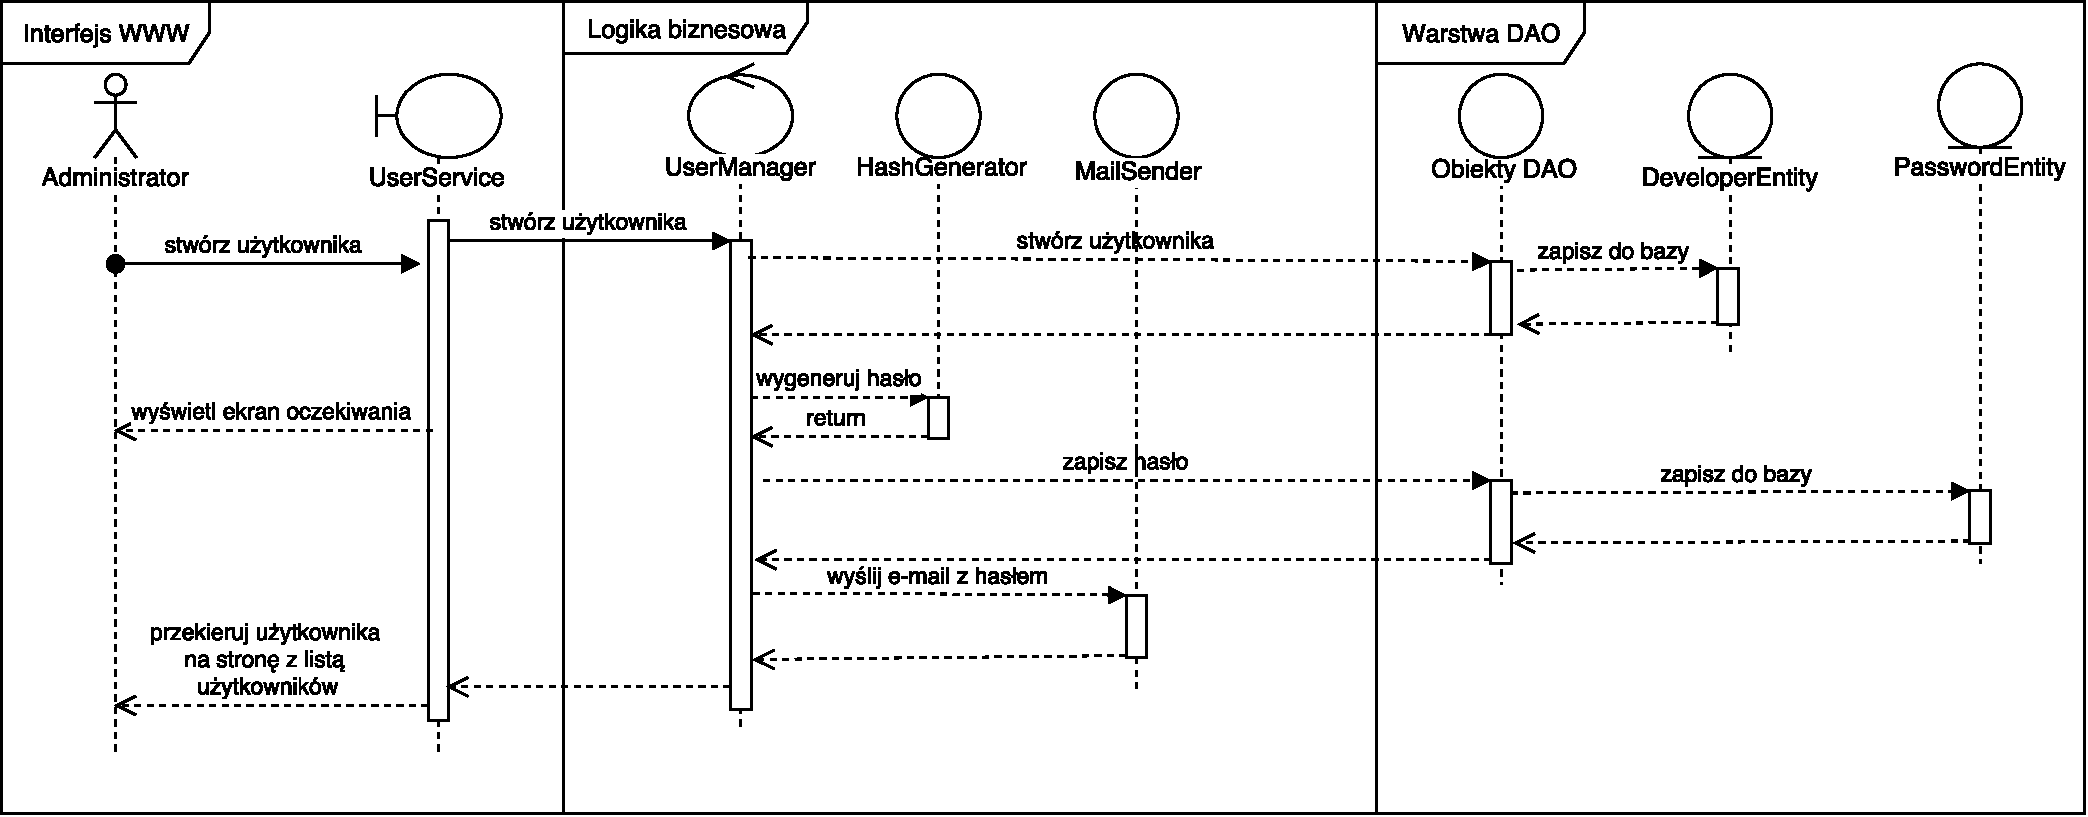
\includegraphics[width=25cm]{rysunki/diagsekw.pdf}	
	\caption{Diagram sekwencji przedstawiający proces tworzenia nowego użytkownika}
	\label{fig:diagsekw}
\end{sidewaysfigure}

Na diagramie nie została uwzględniona operacja anulowania transakcji, ze względu na czytelność. Przerwanie procesu może nastąpić przy zapisywaniu użytkownika do bazy - błąd komunikacji, generowaniu hasła - brak algorytmu SHA-256, zapisywaniu hasła do bazy - błąd komunikacji lub też przy wysyłaniu e-maila z hasłem w sytuacji, gdy wprowadzimy złe ustawienia podczas procesu konfiguracji. W każdym z tych przypadków generowany jest odpowiedni wyjątek, który następnie jest obsługiwany przez warstwę JSF, a użytkownikowi zostaje wyświetlona stosowna informacja.

Generowanie haseł odbywa się poprzez klasę narzędziową UUID z pakietu java.util. Generuje ona co prawda numer UUID, lecz z powodzeniem można go wykorzystać jako hasło początkowe użytkownika, wystarczy tylko usunąć wszystkie znaki myślnika (-) z tak wygenerowanego ciągu znaków. Następnie hasło jest szyfrowane za pomocą algorytmu SHA256 i w takiej postaci jest zapisywane w bazie danych. Cały kod odpowiedzialny za generowanie i szyfrowanie hasła został zamieszony na listingu \ref{lis:generowanie_hasla}.

\begin{lstlisting}[caption={Klasa generująca i szyfrująca hasła}, label=lis:generowanie_hasla, numbers=none]
public class HashGenerator {

public String generateHash() {
return UUID.randomUUID().toString().replaceAll("-", "");
}

public String encodeWithSHA256(String text) 
throws NoSuchAlgorithmException, UnsupportedEncodingException {
return String.format("%064x", new BigInteger(1, 
MessageDigest.getInstance("SHA-256").update(text.getBytes("UTF-8")).digest());
}
}\end{lstlisting}

\subsection{Warstwa prezentacji}

Ostatnią warstwą, która zostanie omówiona w tym rozdziale jest widok użytkownika, czyli warstwa prezentacji. Równolegle z tą warstwą idą w parze usługi REST, za pomocą których można komunikować się z systemem. Są jednak one rozwinięte w bardzo małym stopniu - jedynie w celach demonstracyjnych.

Widoki użytkownika opierają się na technologii JSF 2.2 oraz darmowym frameworku Primefaces w wersji 5.3. Dzięki jego funkcjonalności zostały zaimplementowane tabele, menu, czy różnego rodzaju listy dostępne na stronach systemu. Całość operacji wykonywanych na stronie odbywa się za pomocą JavaScriptu, który został użyty przez framework oraz ziaren Backing Beans. Ziarna te mają dodatkową funkcjonalność - są odpowiedzialne za dostarczanie danych do widoku oraz obsługę żądań - to w nich znajduje się kod, który wykonuje się po wciśnięciu przycisku. Dla przykładu na listingu \ref{lis:kod_form_tworzenia_uzyt} został przedstawiony częściowy kod formularza, napisany w xhtml z użyciem JSF oraz Primefaces odpowiedzialny za wykonanie akcji tworzenia użytkownika. Na listingu został pominięty fragment odpowiedzialny za wyświetlanie pól, w których wprowadza się imię, nazwisko, nazwę użytkownika oraz adres e-mail.

\begin{lstlisting}[caption={Kod formularza tworzenia użytkownika}, label=lis:kod_form_tworzenia_uzyt, numbers=none]
<h:form id="createUserForm">
<p:panel id="createUserPanel" header="#{i18n['page.admin.user.create']}">
<p:focus context="createUserPanel" />
<p:messages id="messages" globalOnly="true closable="true" />
<h:panelGrid columns="3" cellpadding="5">
................
</h:panelGrid>
<p:commandButton id="createButton" value="#{i18n['page.admin.user.create']}"
action="#{userService.createUser}" ajax="false" icon="fa fa-user-plus"
validateClient="true" onclick="PF('block').show()" />
</p:panel>
<p:blockUI block="createUserPanel" trigger="createButton" widgetVar="block">
<p:outputLabel value="#{i18n['page.admin.user.create.process']}" />
<br />
<p:graphicImage library="primefaces" name="/outputpanel/images/loading.gif" />
</p:blockUI>
</h:form>\end{lstlisting}

Najważniejszym elementem kodu jest przycisk utworzony za pomocą znacznika Primefaces <p:commandButton~...~/>. Jego wartość (value), czyli wyświetlany tekst jest pobierany za pomocą zasobu o nazwie \textbf{i18n}, co sprawia, że możliwa jest internacjonalizacja systemu. Ta funkcjonalność również została wykonana w ramach pracy dyplomowej. Kolejnym elementem jest akcja (action) przycisku, która wskazuje na metodę \textit{createUser} z klasy \textit{UserService} zadeklarowanej jako ziarno o zasięgu widoku (view scoped). Po naciśnięciu przycisku zostaje wykonana JavaScriptowa akcja uruchomiona za pomocą obsługi onclick. Jej zadaniem jest wyświetlenie okna poczekania. Krok ten odpowiada wysłaniu żądania utworzenia użytkownika z widoku do ziarna UserService, a następnie wyświetleniu animacji przez ten serwis. Przebieg akcji został przedstawiony we wcześniejszej sekcji na rysunku \ref{fig:diagsekw}. Samo okno poczekania zostało zaprezentowane na ilustracji \ref{fig:user-czekanie}. 
\begin{figure}[h!]
	\centering
	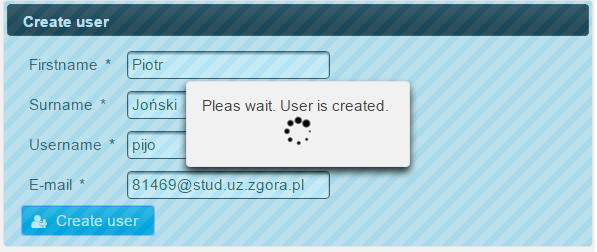
\includegraphics[width=15cm]{rysunki/user-czekanie.png}	
	\caption{Ekran poczekania podczas tworzenia użytkownika}
	\label{fig:user-czekanie}
\end{figure}

\begin{figure}[t]
	\centering
	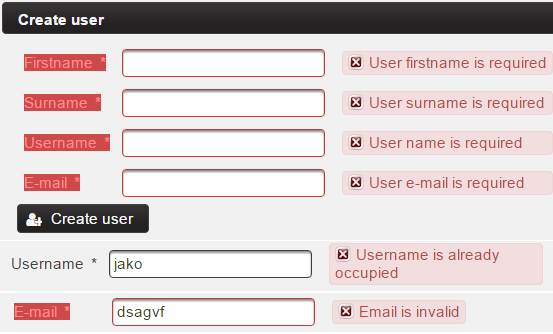
\includegraphics[width=15cm]{rysunki/user-blad.png}	
	\caption{Komunikaty o błędzie podczas tworzenia użytkownika}
	\label{fig:user-blad}
\end{figure}

Po poprawnej walidacji nowy użytkownik zostaje utworzony, na jego skrzynkę trafia e-mail z wygenerowanym hasłem, a administrator zostaje przeniesiony na stronę z listą użytkowników. Jak wiadomo, wprowadzane dane nie zawsze muszą być poprawne. W takim wypadku użytkownikowi zostają wyświetlone komunikaty o błędach, jakie popełnił podczas wprowadzania danych do formularza, co przedstawia rysunek \ref{fig:user-blad}.

Kolejnym aspektem widoku jest to, że został on zaprojektowany w technologi responsywnej, co oznacza, że widok jest skalowany w zależności od rozmiaru okna przeglądarki. Dzięki temu użytkownik zawsze będzie miał wgląd w na całą zawartość strony. To sprawia, że przeglądanie treści systemu jest równie łatwe z poziomu przeglądarek desktopowych jak i urządzeń mobilnych. Technologia ta działa na zasadzie dynamicznego dostosowywania szerokości wyświetlanych elementów i jest w pełni oparta na systemie CSS (Cascading Style Sheets). Została ona zintegrowana z frameworkiem Primefaces, co sprawia, że jej użycie ogranicza się do zastosowania odpowiednich klas komponentów.

System posiada również zabezpieczenia, sprawiające, że część stron jest widoczna tylko dla użytkowników z rolą administratora, a pozostałe treści dla zalogowanych. Zabezpieczenia zostały oparte na specyfikacji JAAS (Java Authentication and Authorization Service), która jest implementowana przez używany kontener - Wildfly. Konfiguracja została przedstawiona na listingu \ref{lis:konf_zab_ad} oraz \ref{lis:konf_zab_zal}.

\begin{lstlisting}[caption={Konfiguracja zabezpieczeń systemu scrumus - administrator}, label=lis:konf_zab_ad, numbers=none]
 <security-constraint>
 <web-resource-collection>
 <web-resource-name>scrumusSecurity</web-resource-name>
 <description>Dostep tylko dla administratora</description>
 <url-pattern>/admin/</url-pattern>
 <http-method>GET</http-method>
 <http-method>POST</http-method>
 <http-method>HEAD</http-method>
 <http-method>PUT</http-method>
 </web-resource-collection>
 <auth-constraint>
 <role-name>ADMIN</role-name>
 </auth-constraint>
 </security-constraint>
 \end{lstlisting}
 \newpage
 \begin{lstlisting}[caption={Konfiguracja zabezpieczeń systemu scrumus - zalogowany użytkownik}, label=lis:konf_zab_zal, numbers=none]
 <security-constraint>
 <web-resource-collection>
 <web-resource-name>scrumusSecurity</web-resource-name>
 <description>Dostep tylko dla zalogowanych uzytkownikow</description>
 <url-pattern>/</url-pattern>
 <http-method>GET</http-method>
 <http-method>POST</http-method>
 <http-method>HEAD</http-method>
 <http-method>PUT</http-method>
 </web-resource-collection>
 <auth-constraint>
 <role-name>DEVELOPER</role-name>
 </auth-constraint>
 </security-constraint>\end{lstlisting}
 
 
 Kolejnym możliwym sposobem komunikacji z aplikacją jest usługa REST, która jest oparta na protokole HTTP. Po wysłaniu zapytania na wybrany adres otrzymujemy odpowiedź w postaci obiektu JSON (JavaScript Object Notation). Protokół HTTP umożliwia różne metody do komunikacji m.in.: GET - pobranie zasobów, POST - wysłanie zapytania z ciałem, które jest używane przy zapisywaniu obiektów oraz DELETE - usuwanie obiektów. Listing \ref{lis:rest} przedstawia konfigurację takiej usługi, która mogłaby zostać zaimplementowana na nowej lub istniejącej już warstwie JSF. Takie rozwiązanie umożliwia rozbudowę systemu o dodatkowe klienty.

\begin{lstlisting}[caption={Przykładowa usługa REST}, label=lis:rest, numbers=none]
@GET
@Path("/users/{userId}")
public Developer findUser(String userId) {
	  try {
	  int userInId = Integer.parseInt(userId);
		  Optional<Developer> userOptional = userManager.findByUserId(userInId);
		  return userOptional.orElse(null);
	  } catch (NumberFormatException e) {
		  return null;
	  }
}
\end{lstlisting}


